%!TEX root = ../slides.tex
\section{Theoretical framework}
\subsection{Stay points}
\begin{frame}{Theoretical framework}{Stay points, Event Driven Systems (EDSs)}
\vspace{-0.2cm}
\small
\begin{block}{\small \textbf{Stay point}}
\begin{itemize}
  \item A stay point refers to a geographical zone (of size $\delta_{distance}$) where the user remains for an amount of time ($\delta_{time}$).
  \item It is a virtual location defined by latitude (\emph{lat}), longitude (\emph{lon}), arrival time (\emph{at}) and departure time (\emph{dt}).
\end{itemize}
\end{block}

\vspace{-0.2cm}
\begin{columns}
\begin{column}{0.5\textwidth}
\begin{block}{\small \textbf{Event Driven Systems (EDSs)}}
{
    \centering
    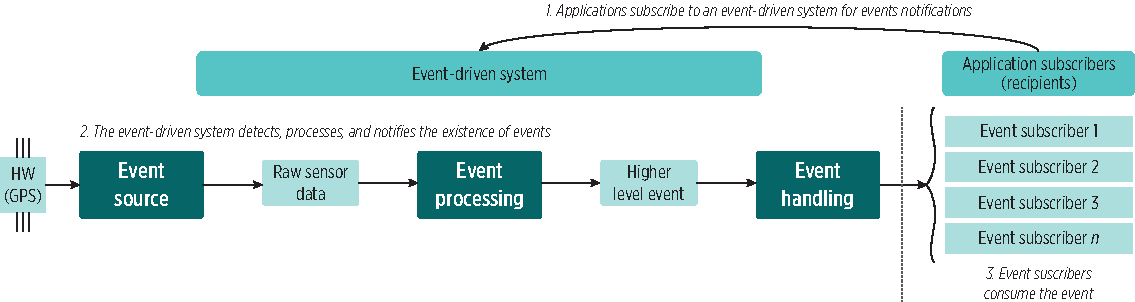
\includegraphics[width=0.55\textwidth]{vectors/event-driven-system-for-slides}
    \captionof{figure}{The architecture of an EDS.}
    \par
}
\end{block}
\end{column}

\begin{column}{0.5\textwidth}
\begin{block}{\small \textbf{Cognitive Dynamic Systems (CDSs)}}
\begin{figure}
    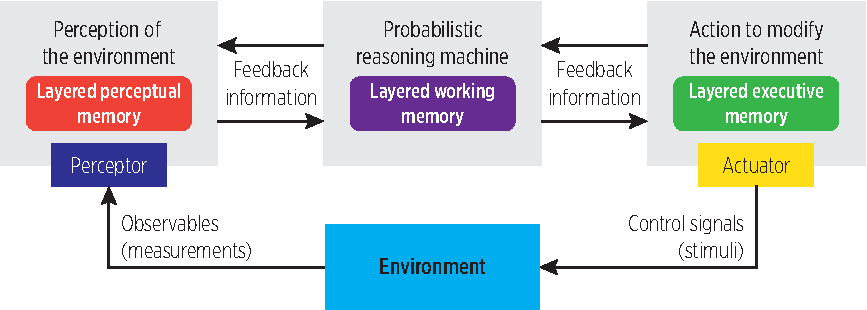
\includegraphics[width=0.53\textwidth]{vectors/cds-adaptation-figure-for-slides}
    \caption{The generic architecture of a CDS.}
\end{figure}
\end{block}
\end{column}
\end{columns}
\end{frame}